\chapter{Overview}
\label{ch:overview}

In this thesis, we present a design for an extension that enhances memory safety in \ac{WASM} built on top of the \ac{WASM} 64-bit memory proposal\footnote{\url{https://github.com/WebAssembly/memory64}}.
The extension is created to be minimally invasive and implementable using various techniques, including hardware extensions such as \ac{MTE} or \ac{PAC}, capability-based architectures like \ac{CHERI}~\cite{woodruff2014cheri}, or software-based solutions similar to \ac{ASAN}~\cite{serebryany2012addresssanitizer} or \ac{HWASAN}~\cite{serebryany2018memory} (see \cref{ch:design}).


\begin{figure}[ht]
    \centering
    % not the best name lmao
    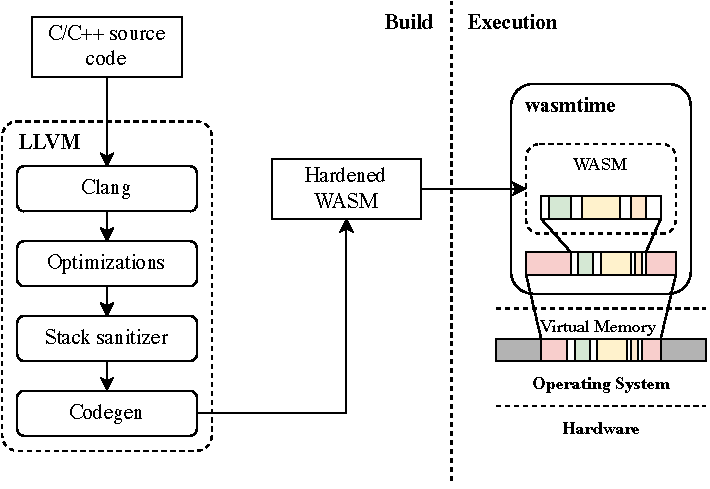
\includegraphics{figures/build/overview-simple}
    \caption{Overview of the prototype implemented in this thesis.}
    \label{fig:system-overview}
\end{figure}

In \cref{fig:system-overview}, we present our prototype of this design.
Unmodified C/C++ source code is compiled using LLVM~\cite{lattner2004llvm}, where we implement a sanitizer that identifies and hardens stack allocations, along with a modified standard library based on \ac{WASI} that protects heap allocations.
LLVM then generates hardened \ac{WASM} binaries that can be run in wasmtime\footnote{\url{https://wasmtime.dev/}}.
We modify wasmtime to process our \ac{WASM} extension and implement it using \ac{MTE}.

Additionally, we explore and implement a technique to efficiently sandbox \ac{WASM} programs using \ac{MTE}, eliminating expensive software-based bounds checks required for 64-bit \ac{WASM} programs.
This technique can be combined with the \ac{MTE}-based memory safety implementation.

We analyze and benchmark various aspects of our implementation, including 32-bit and 64-bit \ac{WASM}, and the \ac{MTE} implementation on real hardware (see \cref{ch:eval}).
